% ------------------------------------------------------------------ %
%  CentralImmo -- Rapport d'architecture et de conception
%  Diagrammes r\'ealis\'es avec TikZ / tkz (TeX Live 2025)
%  Compilation : pdflatex report.tex (deux passes recommandees)
% ------------------------------------------------------------------ %
\documentclass[11pt,a4paper]{report}

\usepackage[utf8]{inputenc}
\usepackage[T1]{fontenc}
\usepackage[margin=2.2cm,top=2.4cm,bottom=2.4cm]{geometry}
\usepackage{xcolor}
\usepackage{tikz}
\usepackage{tkz-graph}
\usepackage{tkz-tab}
\usepackage{caption}
\usepackage{float}
\usepackage{titlesec}
\usepackage{enumitem}
\usepackage{booktabs}
\usepackage{hyperref}

\hypersetup{
  colorlinks=true,
  linkcolor=black,
  urlcolor=black,
  pdftitle={CentralImmo -- Rapport d'architecture},
  pdfauthor={CentralImmo}
}

% TikZ libraries
\usetikzlibrary{positioning,arrows.meta,shapes.geometric,fit,calc,
  backgrounds,shadows,decorations.pathreplacing,decorations.pathmorphing,
  shapes.misc,shapes.symbols,automata,positioning}

% --- Palette CentralImmo ---
\definecolor{ciOrange}{HTML}{E94E1B}
\definecolor{ciOrangeL}{HTML}{F7B59A}
\definecolor{ciBlue}{HTML}{1F4E79}
\definecolor{ciBlueL}{HTML}{C7DCEF}
\definecolor{ciGreen}{HTML}{2E7D32}
\definecolor{ciGreenL}{HTML}{C8E6C9}
\definecolor{ciGray}{HTML}{4A4A4A}
\definecolor{ciGrayL}{HTML}{ECECEC}
\definecolor{ciPurple}{HTML}{5E35B1}
\definecolor{ciPurpleL}{HTML}{D5C5F0}
\definecolor{ciRed}{HTML}{B00020}
\definecolor{ciAmber}{HTML}{F59E0B}
\definecolor{ciAmberL}{HTML}{FDE9C7}
\definecolor{ciAws}{HTML}{FF9900}
\definecolor{ciAwsD}{HTML}{232F3E}
\definecolor{ciWhite}{HTML}{FFFFFF}

% Styles TikZ globaux
\tikzset{
  ci-box/.style={
    draw=ciGray, line width=0.6pt, rounded corners=3pt,
    fill=ciWhite, font=\small\sffamily, align=center,
    inner sep=6pt, minimum height=8mm
  },
  ci-orange/.style={ci-box, draw=ciOrange, fill=ciOrangeL!40},
  ci-blue/.style={ci-box, draw=ciBlue, fill=ciBlueL!50},
  ci-green/.style={ci-box, draw=ciGreen, fill=ciGreenL!60},
  ci-purple/.style={ci-box, draw=ciPurple, fill=ciPurpleL!50},
  ci-amber/.style={ci-box, draw=ciAmber!80!black, fill=ciAmberL!70},
  ci-gray/.style={ci-box, draw=ciGray, fill=ciGrayL},
  ci-aws/.style={ci-box, draw=ciAwsD, fill=ciAws!20},
  ci-flow/.style={-Stealth, line width=0.8pt, draw=ciGray},
  ci-flow-d/.style={-Stealth, line width=0.8pt, draw=ciOrange, dashed},
  ci-label/.style={font=\footnotesize\sffamily, midway, fill=ciWhite,
    inner sep=2pt, text=ciGray},
  ci-title/.style={font=\small\bfseries\sffamily, text=ciBlue}
}

\titleformat{\chapter}[display]
  {\normalfont\huge\bfseries\color{ciOrange}}{\chaptername\ \thechapter}{20pt}{\Huge}
\titleformat{\section}{\normalfont\large\bfseries\color{ciBlue}}{\thesection}{1em}{}
\setlength{\parindent}{0pt}

% French labels (no babel available)
\renewcommand{\chaptername}{Chapitre}
\renewcommand{\contentsname}{Table des mati\`eres}
\renewcommand{\figurename}{Figure}
\renewcommand{\tablename}{Tableau}
\renewcommand{\abstractname}{R\'esum\'e}

\title{\bfseries CentralImmo \\ \large Rapport d'architecture et de conception}
\author{P\'eronnal}
\date{Juin 2026}

\begin{document}
\maketitle
\thispagestyle{empty}

\begin{abstract}
\noindent
CentralImmo est une plateforme d'agr\'egation immobili\`ere et d'intelligence
de march\'e pour le Cameroun. Le pr\'esent rapport illustre l'architecture
g\'en\'erale du syst\`eme au moyen de onze diagrammes r\'ealis\'es en TikZ~:
architecture g\'en\'erale, d\'eploiement AWS EC2, mod\`ele de donn\'ees,
framework de scraping, pipeline d'ingestion, orchestration des crawls,
r\'esolution des doublons (DCS), scraper universel, pipeline analytique,
flux de requ\^etes API et machine \`a \'etats du review des annonces.
Le backend FastAPI est h\'eberg\'e sur une instance AWS EC2, avec une base
PostgreSQL manag\'ee par Amazon RDS, derri\`ere un \'equilibreur de charge
Application Load Balancer et une distribution CloudFront pour le front web.
\end{abstract}

\tableofcontents

% ================================================================== %
\chapter{Architecture g\'en\'erale du syst\`eme}
% ================================================================== %

La plateforme s'organise en quatre plans fonctionnels~: la collecte
(scrapers Python), la persistance (PostgreSQL multi-couches), l'API
(FastAPI) et la pr\'esentation (Flutter multi-plateforme). Le scheduler
APScheduler s'ex\'ecute en arri\`ere-plan au sein du processus FastAPI.

\begin{figure}[H]
\centering
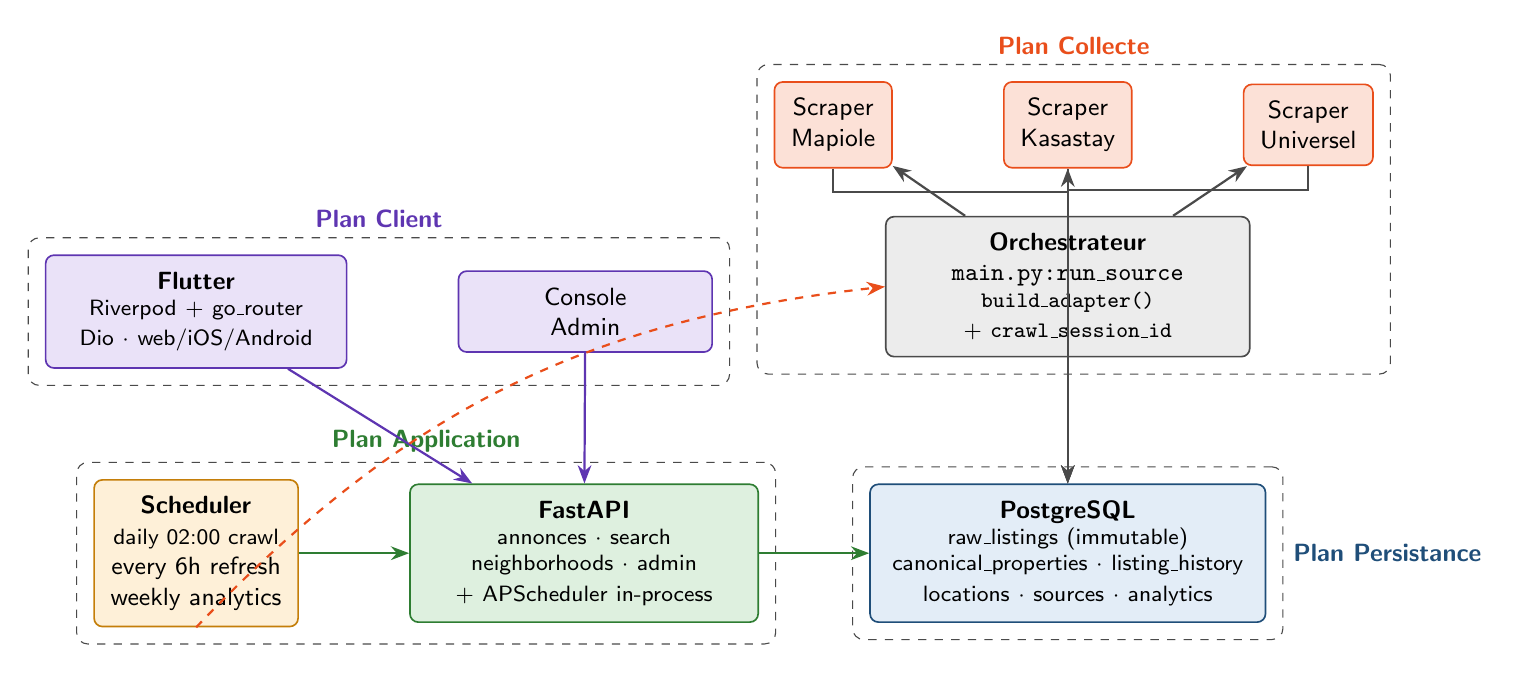
\begin{tikzpicture}[
  node distance=10mm and 14mm,
  layer/.style={draw=ciGray, dashed, rounded corners=4pt,
    inner sep=6pt, font=\small\bfseries\sffamily, text=ciGray}
]
% --- Plan Collecte ---
\node[ci-orange] (mapiole) {Scraper\\Mapiole};
\node[ci-orange, right=of mapiole] (kasastay) {Scraper\\Kasastay};
\node[ci-orange, right=of kasastay] (universal) {Scraper\\Universel};
\node[ci-gray, below=6mm of kasastay, text width=42mm]
  (orchestrator) {\textbf{Orchestrateur}\\ \texttt{main.py:run\_source}\\
  \footnotesize \texttt{build\_adapter()} \\+ \texttt{crawl\_session\_id}};

\node[layer, fit=(mapiole) (kasastay) (universal) (orchestrator),
  label={[font=\small\bfseries\sffamily,color=ciOrange]above:Plan Collecte}] (L1) {};

% --- Plan Persistance ---
\node[ci-blue, below=16mm of orchestrator, text width=46mm]
  (db) {\textbf{PostgreSQL}\\
  \footnotesize raw\_listings (immutable)\\
  canonical\_properties $\cdot$ listing\_history\\
  locations $\cdot$ sources $\cdot$ analytics};
\node[layer, fit=(db),
  label={[font=\small\bfseries\sffamily,color=ciBlue]right:Plan Persistance}] {};

% --- Plan API ---
\node[ci-green, left=14mm of db, text width=40mm]
  (api) {\textbf{FastAPI}\\ \footnotesize annonces $\cdot$ search\\
  neighborhoods $\cdot$ admin\\ \footnotesize + APScheduler in-process};
\node[ci-amber, left=14mm of api] (sched)
  {\textbf{Scheduler}\\ \footnotesize daily 02:00 crawl\\
  every 6h refresh\\ weekly analytics};
\node[layer, fit=(api) (sched),
  label={[font=\small\bfseries\sffamily,color=ciGreen]above:Plan Application}] {};

% --- Plan Pr\'esentation ---
\node[ci-purple, above=14mm of sched, text width=34mm]
  (flutter) {\textbf{Flutter}\\ \footnotesize Riverpod + go\_router\\
  Dio $\cdot$ web/iOS/Android};
\node[ci-purple, right=of flutter, text width=28mm]
  (adminui) {Console\\Admin};
\node[layer, fit=(flutter) (adminui),
  label={[font=\small\bfseries\sffamily,color=ciPurple]above:Plan Client}] {};

% --- Flux ---
\draw[ci-flow] (orchestrator) -- (mapiole);
\draw[ci-flow] (orchestrator) -- (kasastay);
\draw[ci-flow] (orchestrator) -- (universal);
\draw[ci-flow] (mapiole.south) -- ++(0,-3mm) -| (db.north);
\draw[ci-flow] (kasastay.south) -- ++(0,-3mm) -| (db.north);
\draw[ci-flow] (universal.south) -- ++(0,-3mm) -| (db.north);
\draw[ci-flow, draw=ciGreen] (api) -- (db);
\draw[ci-flow, draw=ciGreen] (sched) -- (api);
\draw[ci-flow, draw=ciPurple] (flutter) -- (api);
\draw[ci-flow, draw=ciPurple] (adminui) -- (api);
\draw[ci-flow-d] (sched.south) to[bend left=20] (orchestrator.west);
\end{tikzpicture}
\caption{Architecture en quatre plans de CentralImmo.}
\end{figure}

% ================================================================== %
\chapter{D\'eploiement sur AWS EC2}
% ================================================================== %

Le backend FastAPI est h\'eberg\'e sur une instance EC2 (Amazon Linux 2023,
type \texttt{t3.medium}) dans un VPC priv\'e. La base PostgreSQL est d\'el\'egu\'ee
\`a Amazon RDS pour la sauvegarde automatique et le bascuement multi-AZ.
La distribution CloudFront sert le build web Flutter et met en cache les
images d'annonces. Route~53 r\'esout \texttt{centralimmo.cm} vers l'ALB.

\begin{figure}[H]
\centering
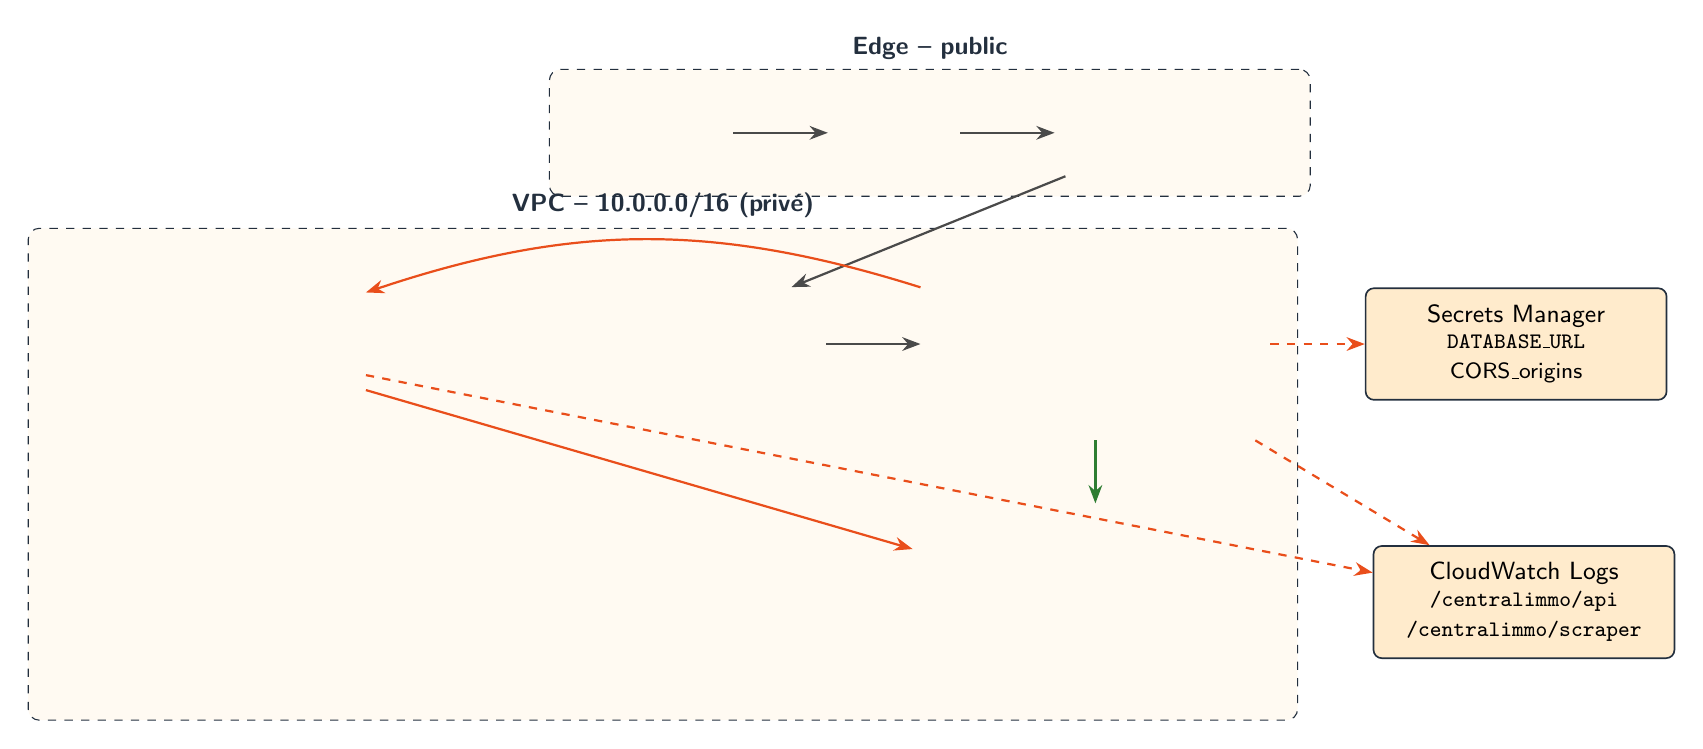
\begin{tikzpicture}[
  node distance=7mm and 12mm,
  aws-group/.style={draw=ciAwsD, dashed, rounded corners=4pt,
    inner sep=7pt, font=\small\bfseries\sffamily, text=ciAwsD, fill=ciAws!5}
]
% Edge
\node[ci-aws] (user) {Utilisateurs\\ \footnotesize mobile / web};
\node[ci-aws, right=of user] (dns) {Route 53\\ \footnotesize DNS};
\node[ci-aws, right=of dns] (cdn) {CloudFront\\ \footnotesize cache web + images};
\node[aws-group, fit=(user)(dns)(cdn),
  label={[font=\small\bfseries\sffamily,color=ciAwsD]above:Edge -- public}] {};

% VPC
\node[ci-aws, below=14mm of user, text width=40mm] (alb)
  {Application Load Balancer\\ \footnotesize HTTPS:443 $\to$ 8000\\
  SG: \texttt{sg-alb}};
\node[ci-aws, right=of alb, text width=40mm] (ec2)
  {\textbf{EC2 t3.medium}\\ \footnotesize Amazon Linux 2023\\
  systemd \texttt{centralimmo.service}\\ uvicorn + gunicorn (4 workers)\\
  FastAPI + APScheduler\\ SG: \texttt{sg-app}};
\node[ci-aws, below=8mm of ec2, text width=42mm] (rds)
  {Amazon RDS PostgreSQL 16\\ \footnotesize db.t4g.medium, multi-AZ\\
  encrypted at rest, automated backup\\ SG: \texttt{sg-db} (ingress 5432 from sg-app)};

\node[ci-aws, left=14mm of alb, text width=36mm] (scraper)
  {Scraper workers\\ \footnotesize m\^eme processus que FastAPI\\
  cron: 02:00 / 6h / lun 03:00};

\node[aws-group, fit=(alb)(ec2)(rds)(scraper),
  label={[font=\small\bfseries\sffamily,color=ciAwsD]above:VPC -- 10.0.0.0/16 (priv\'e)}] (vpc) {};

% Secret manager + logs
\node[ci-aws, right=12mm of ec2, text width=34mm] (sm)
  {Secrets Manager\\ \footnotesize \texttt{DATABASE\_URL}\\ CORS\_origins};
\node[ci-aws, right=12mm of rds, text width=34mm] (logs)
  {CloudWatch Logs\\ \footnotesize \texttt{/centralimmo/api}\\
  \texttt{/centralimmo/scraper}};

\draw[ci-flow] (user) -- (dns);
\draw[ci-flow] (dns) -- (cdn);
\draw[ci-flow] (cdn) -- (alb);
\draw[ci-flow] (alb) -- (ec2);
\draw[ci-flow, draw=ciGreen] (ec2) -- (rds);
\draw[ci-flow, draw=ciOrange] (scraper) -- (rds);
\draw[ci-flow, draw=ciOrange] (ec2) to[bend right=18] (scraper);
\draw[ci-flow-d] (ec2) -- (sm);
\draw[ci-flow-d] (ec2) -- (logs);
\draw[ci-flow-d] (scraper) -- (logs);
\end{tikzpicture}
\caption{Topologie de d\'eploiement sur AWS (EC2 + RDS + CloudFront).}
\end{figure}

% ================================================================== %
\chapter{Mod\`ele de donn\'ees (ER)}
% ================================================================== %

Huit tables structurent la persistance~: deux de r\'ef\'erence
(\texttt{sources}, \texttt{locations}), trois c\^ur (\texttt{raw\_listings},
\texttt{canonical\_properties}, \texttt{listing\_history}) et trois
op\'erationnelles (\texttt{image\_cache}, \texttt{scheduler\_jobs},
\texttt{neighborhood\_analytics}). Les r\`egles d'immutabilit\'e et
d'append-only sont mat\'erialis\'ees par les cardinalit\'es.

\begin{figure}[H]
\centering
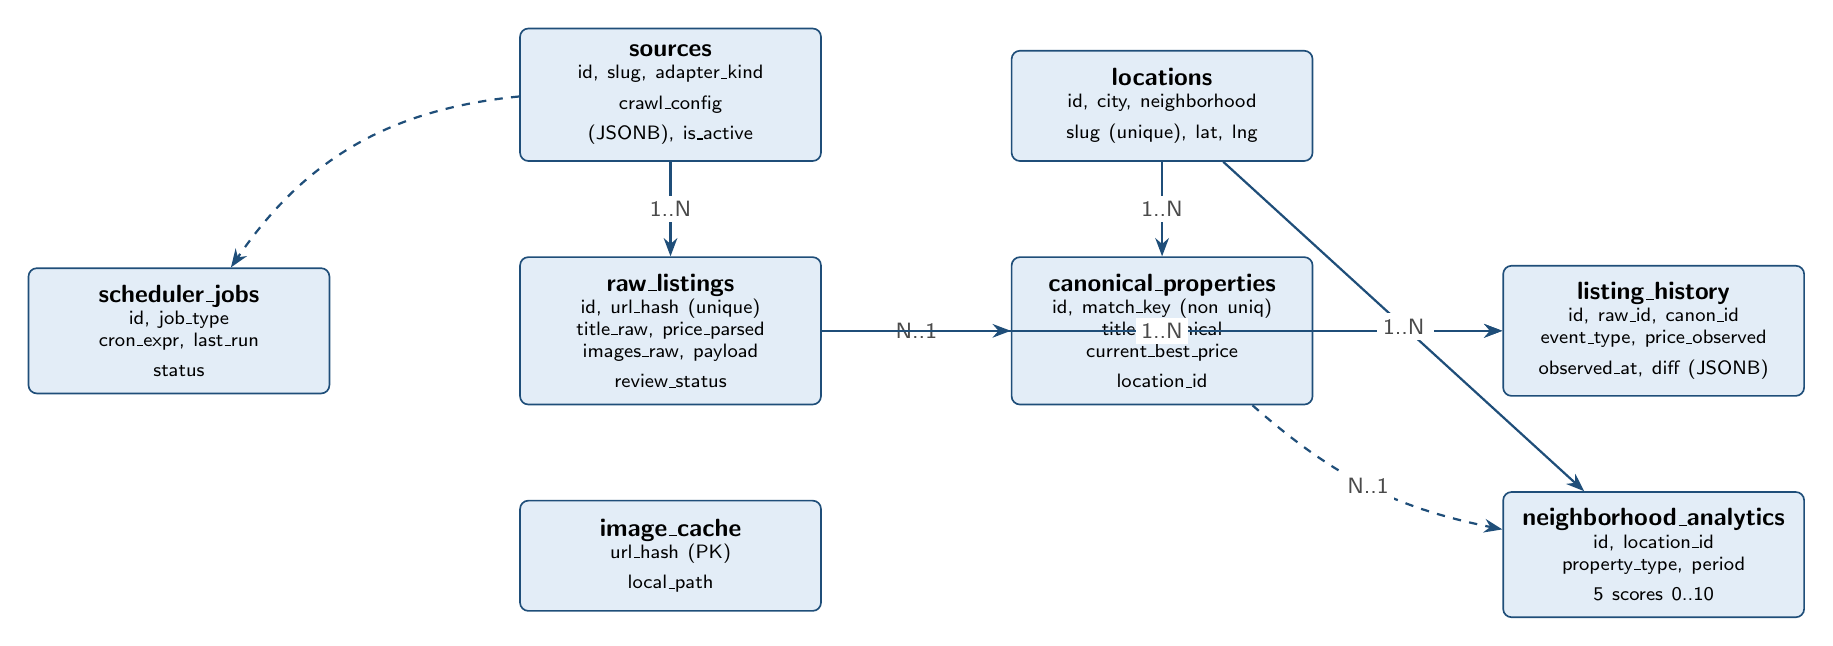
\begin{tikzpicture}[
  node distance=12mm and 24mm,
  ent/.style={ci-blue, text width=34mm, align=center,
    font=\small\sffamily, minimum height=14mm},
  pk/.style={font=\scriptsize\bfseries\sffamily, text=ciOrange}
]
\node[ent] (sources) {\textbf{sources}\\ \scriptsize id, slug, adapter\_kind\\
  crawl\_config (JSONB), is\_active};
\node[ent, below=of sources] (raw)
  {\textbf{raw\_listings}\\ \scriptsize id, url\_hash (unique)\\
  title\_raw, price\_parsed\\ images\_raw, payload\\ review\_status};
\node[ent, right=of raw] (canon)
  {\textbf{canonical\_properties}\\ \scriptsize id, match\_key (non uniq)\\
  title\_canonical\\ current\_best\_price\\ location\_id};
\node[ent, right=of canon] (hist)
  {\textbf{listing\_history}\\ \scriptsize id, raw\_id, canon\_id\\
  event\_type, price\_observed\\ observed\_at, diff (JSONB)};
\node[ent, above=of canon] (loc)
  {\textbf{locations}\\ \scriptsize id, city, neighborhood\\
  slug (unique), lat, lng};
\node[ent, below=of raw] (img)
  {\textbf{image\_cache}\\ \scriptsize url\_hash (PK)\\ local\_path};
\node[ent, below=of hist] (ana)
  {\textbf{neighborhood\_analytics}\\ \scriptsize id, location\_id\\
  property\_type, period\\ 5 scores 0..10};
\node[ent, left=of raw] (jobs)
  {\textbf{scheduler\_jobs}\\ \scriptsize id, job\_type\\
  cron\_expr, last\_run\\ status};

% Relations
\draw[ci-flow, draw=ciBlue] (sources) -- node[ci-label]{1..N} (raw);
\draw[ci-flow, draw=ciBlue] (loc) -- node[ci-label]{1..N} (canon);
\draw[ci-flow, draw=ciBlue] (raw) -- node[ci-label]{N..1} (canon);
\draw[ci-flow, draw=ciBlue] (raw) -- node[ci-label]{1..N} (hist);
\draw[ci-flow, draw=ciBlue] (canon) -- node[ci-label]{1..N} (hist);
\draw[ci-flow, draw=ciBlue] (loc) -- node[ci-label]{1..N} (ana);
\draw[ci-flow-d, draw=ciBlue] (canon) to[bend right=15] node[ci-label]{N..1} (ana);
\draw[ci-flow-d, draw=ciBlue] (sources) to[bend right=25] (jobs);
\end{tikzpicture}
\caption{Sch\'ema entit\'e-association (PK en orange, FK en bleu).}
\end{figure}

% ================================================================== %
\chapter{Framework de scraping}
% ================================================================== %

Tous les adaptateurs impl\'ementent l'ABC \texttt{SourceAdapter}
(\texttt{fetch\_listings}, \texttt{fetch\_details}, \texttt{normalize\_data},
\texttt{validate\_data}) et h\'eritent de \texttt{BaseFetchMixin} pour la
couche HTTP anti-bot. Le scraper universel s'appuie sur les modules
\texttt{extractors} et \texttt{confidence}.

\begin{figure}[H]
\centering
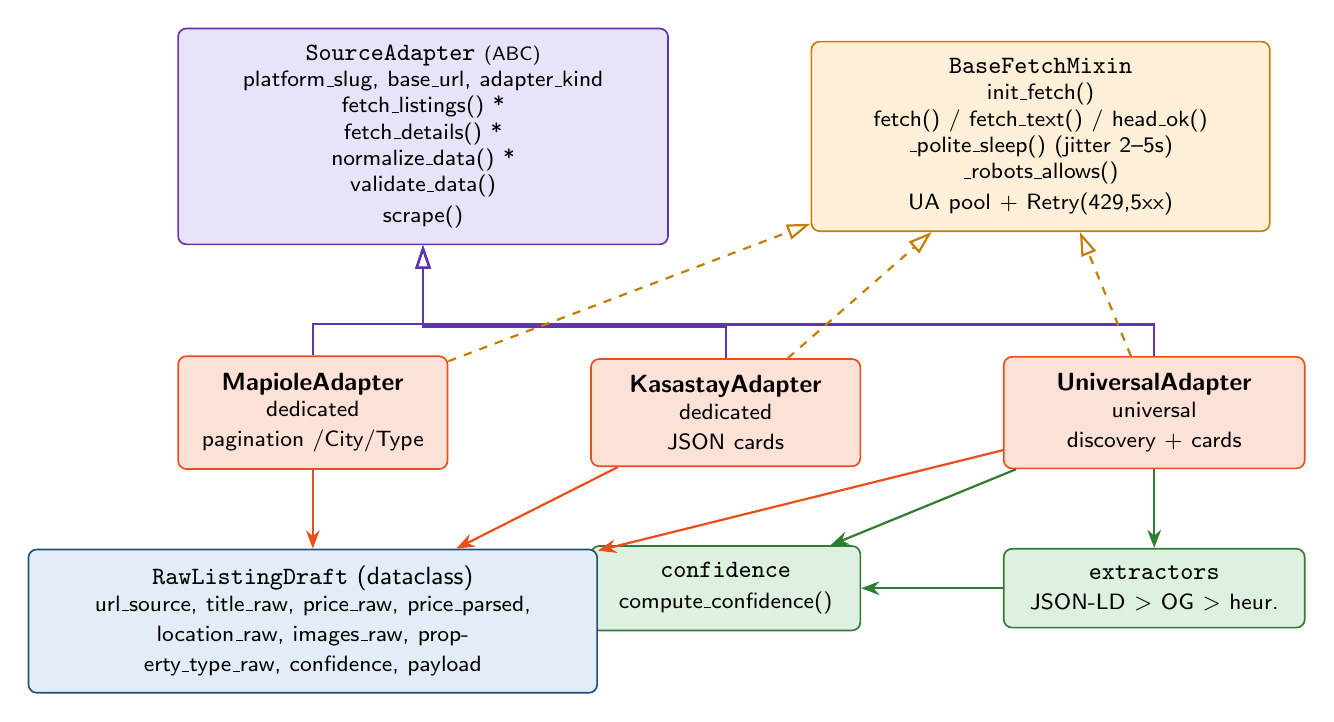
\begin{tikzpicture}[node distance=8mm and 18mm]
% ABC
\node[ci-purple, text width=58mm] (abc)
  {\textbf{\texttt{SourceAdapter}} \scriptsize(ABC)\\
  \footnotesize platform\_slug, base\_url, adapter\_kind\\
  \footnotesize fetch\_listings() *\\
  \footnotesize fetch\_details() *\\
  \footnotesize normalize\_data() *\\
  \footnotesize validate\_data()\\
  \footnotesize scrape()};

% Mixin
\node[ci-amber, right=18mm of abc, text width=54mm] (mix)
  {\textbf{\texttt{BaseFetchMixin}}\\
  \footnotesize init\_fetch()\\
  \footnotesize fetch() / fetch\_text() / head\_ok()\\
  \footnotesize \_polite\_sleep() (jitter 2--5s)\\
  \footnotesize \_robots\_allows()\\
  \footnotesize UA pool + Retry(429,5xx)};

% Subclasses
\node[ci-orange, below=14mm of abc.south west, anchor=north west, text width=30mm]
  (mapiole) {\textbf{MapioleAdapter}\\ \footnotesize dedicated\\ pagination /City/Type};
\node[ci-orange, right=of mapiole, text width=30mm]
  (kasa) {\textbf{KasastayAdapter}\\ \footnotesize dedicated\\ JSON cards};
\node[ci-orange, right=of kasa, text width=34mm]
  (uni) {\textbf{UniversalAdapter}\\ \footnotesize universal\\ discovery + cards};

% Helpers
\node[ci-green, below=10mm of uni, text width=34mm] (extr)
  {\texttt{extractors}\\ \footnotesize JSON-LD $>$ OG $>$ heur.};
\node[ci-green, left=of extr, text width=30mm] (conf)
  {\texttt{confidence}\\ \footnotesize compute\_confidence()};

% Draft
\node[ci-blue, below=10mm of mapiole, text width=68mm] (draft)
  {\textbf{\texttt{RawListingDraft}} (dataclass)\\
  \footnotesize url\_source, title\_raw, price\_raw, price\_parsed,\\
  location\_raw, images\_raw, property\_type\_raw, confidence, payload};

% Relations
\draw[ci-flow, draw=ciPurple, -{Triangle[open, length=3mm]}]
  (mapiole.north) -- ++(0,4mm) -| (abc.south);
\draw[ci-flow, draw=ciPurple, -{Triangle[open, length=3mm]}]
  (kasa.north) -- ++(0,4mm) -| (abc.south);
\draw[ci-flow, draw=ciPurple, -{Triangle[open, length=3mm]}]
  (uni.north) -- ++(0,4mm) -| (abc.south);

\draw[ci-flow, draw=ciAmber!80!black, dashed,
  -{Triangle[open, length=3mm]}] (mapiole) -- (mix);
\draw[ci-flow, draw=ciAmber!80!black, dashed,
  -{Triangle[open, length=3mm]}] (kasa) -- (mix);
\draw[ci-flow, draw=ciAmber!80!black, dashed,
  -{Triangle[open, length=3mm]}] (uni) -- (mix);

\draw[ci-flow, draw=ciGreen] (uni) -- (extr);
\draw[ci-flow, draw=ciGreen] (uni) -- (conf);
\draw[ci-flow, draw=ciGreen] (extr) -- (conf);

\draw[ci-flow, draw=ciOrange] (mapiole) -- (draft);
\draw[ci-flow, draw=ciOrange] (kasa) -- (draft);
\draw[ci-flow, draw=ciOrange] (uni) -- (draft);
\end{tikzpicture}
\caption{Hi\'erarchie d'adaptateurs et mixin anti-bot.}
\end{figure}

% ================================================================== %
\chapter{Pipeline d'ingestion}
% ================================================================== %

\texttt{core/ingest.py} transforme les \texttt{RawListingDraft} en lignes
\texttt{raw\_listings} + \texttt{canonical\_properties} +
\texttt{listing\_history}. L'idempotence est garantie par
\texttt{url\_hash = sha256(url\_source)}~: un re-crawl ne cr\'ee jamais de
nouvelle ligne, il compare le prix \`a la derni\`ere \texttt{listing\_history}
et n'ajoute un \'ev\'enement \texttt{price\_change} que si la valeur a boug\'e.

\begin{figure}[H]
\centering
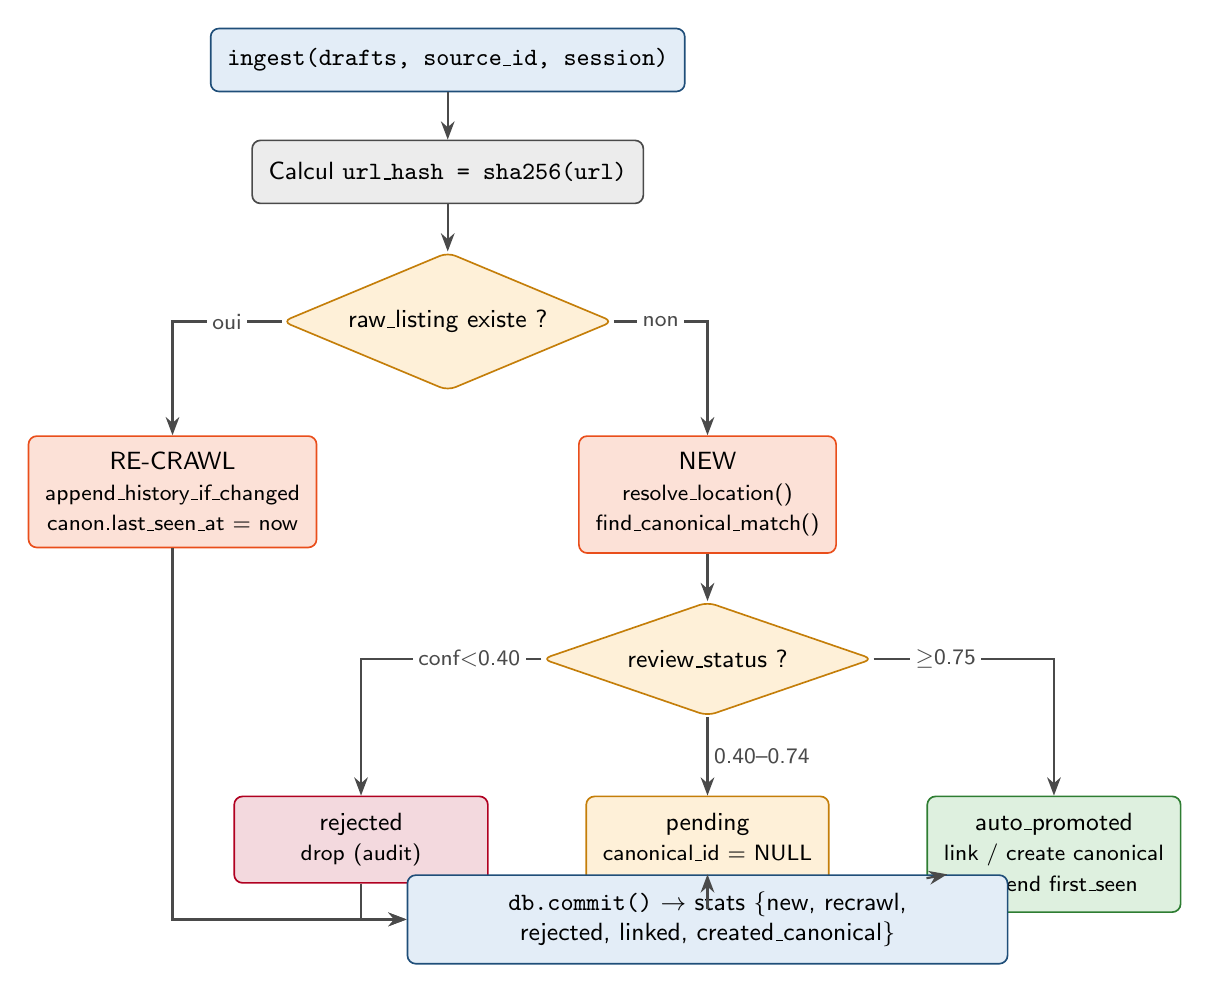
\begin{tikzpicture}[
  node distance=6mm and 14mm,
  dec/.style={ci-amber, diamond, aspect=2, inner sep=2pt,
    minimum width=42mm, minimum height=12mm, font=\small\sffamily}
]
\node[ci-blue] (in) {\texttt{ingest(drafts, source\_id, session)}};
\node[ci-gray, below=of in] (hash)
  {Calcul \texttt{url\_hash = sha256(url)}};
\node[dec, below=of hash] (exists) {raw\_listing existe ?};
\node[ci-orange, below left=10mm and 6mm of exists] (recrawl)
  {RE-CRAWL\\ \footnotesize append\_history\_if\_changed\\
  \footnotesize canon.last\_seen\_at = now};
\node[ci-orange, below right=10mm and 6mm of exists] (new)
  {NEW\\ \footnotesize resolve\_location()\\
  \footnotesize find\_canonical\_match()};
\node[dec, below=of new] (status) {review\_status ?};
\node[ci-box, draw=ciRed, fill=ciRed!15,
  below=10mm of status, xshift=-44mm, text width=28mm] (rej)
  {rejected\\ \footnotesize drop (audit)};
\node[ci-amber, below=10mm of status] (pend)
  {pending\\ \footnotesize canonical\_id = NULL\\
  \footnotesize attente admin review};
\node[ci-green, below=10mm of status, xshift=44mm] (prom)
  {auto\_promoted\\ \footnotesize link / create canonical\\
  \footnotesize append first\_seen};
\node[ci-blue, below=20mm of status, text width=72mm] (commit)
  {\texttt{db.commit()} $\to$ stats \{new, recrawl, rejected, linked, created\_canonical\}};

\draw[ci-flow] (in) -- (hash);
\draw[ci-flow] (hash) -- (exists);
\draw[ci-flow] (exists) -| node[ci-label,pos=0.25]{oui} (recrawl);
\draw[ci-flow] (exists) -| node[ci-label,pos=0.25]{non} (new);
\draw[ci-flow] (new) -- (status);
\draw[ci-flow] (status) -| node[ci-label,pos=0.2]{conf$<$0.40} (rej);
\draw[ci-flow] (status) -- node[ci-label,right]{0.40--0.74} (pend);
\draw[ci-flow] (status) -| node[ci-label,pos=0.2]{$\geq$0.75} (prom);
\draw[ci-flow] (recrawl) |- (commit);
\draw[ci-flow] (rej) |- (commit);
\draw[ci-flow] (pend) -- (commit);
\draw[ci-flow] (prom) -- (commit);
\end{tikzpicture}
\caption{Logique d'ingestion idempotente (re-crawl vs nouveau).}
\end{figure}

% ================================================================== %
\chapter{Orchestration des crawls (s\'equence)}
% ================================================================== %

La s\'equence ci-dessous d\'ecrit l'ex\'ecution d'une source par le
scheduler (cron quotidien 02:00 UTC) ou par appel manuel
\texttt{POST /admin/sources/\{slug\}/crawl}.

\begin{figure}[H]
\centering
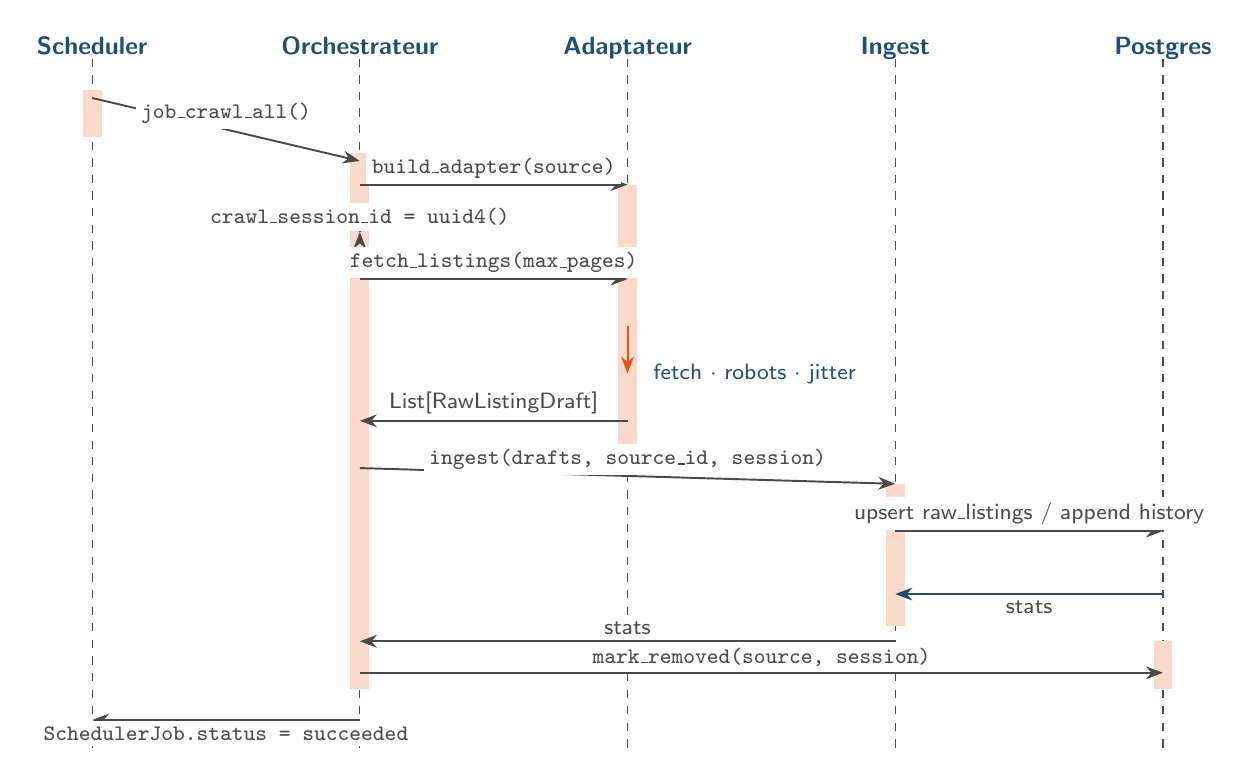
\begin{tikzpicture}[
  node distance=4mm,
  life/.style={draw=ciGray, line width=0.4pt, dashed},
  act/.style={font=\footnotesize\sffamily, text=ciBlue, align=left},
  msg/.style={-Stealth, line width=0.7pt, draw=ciGray,
    font=\scriptsize\sffamily}
]
% Lifelines
\foreach \x/\n in {0/Scheduler, 3.4/Orchestrateur, 6.8/Adaptateur, 10.2/Ingest, 13.6/Postgres}{
  \node[ci-title, anchor=north] at (\x,0) {\n};
  \draw[life] (\x,-0.4) -- (\x,-9.2);
}
% Activations (rectangles)
\foreach \x/\ya/\yb in {0/-0.8/-1.4, 3.4/-1.6/-8.4, 6.8/-2.0/-5.6, 10.2/-5.8/-7.6, 13.6/-7.8/-8.4}{
  \fill[ciOrangeL!50] (\x-0.12,\ya) rectangle (\x+0.12,\yb);
}
% Messages
\draw[msg] (0,-0.9) -- node[ci-label,above]{\texttt{job\_crawl\_all()}} (3.4,-1.7);
\draw[msg] (3.4,-2.0) -- node[ci-label,above]{\texttt{build\_adapter(source)}} (6.8,-2.0);
\draw[msg] (3.4,-2.6) -- node[ci-label,above]{\texttt{crawl\_session\_id = uuid4()}} (3.4,-2.6);
\draw[msg] (3.4,-3.2) -- node[ci-label,above]{\texttt{fetch\_listings(max\_pages)}} (6.8,-3.2);
\draw[msg, draw=ciOrange] (6.8,-3.8) -- ++(0,-0.6) node[act,right=2mm]{fetch $\cdot$ robots $\cdot$ jitter};
\draw[msg] (6.8,-5.0) -- node[ci-label,above]{List[RawListingDraft]} (3.4,-5.0);
\draw[msg] (3.4,-5.6) -- node[ci-label,above]{\texttt{ingest(drafts, source\_id, session)}} (10.2,-5.8);
\draw[msg] (10.2,-6.4) -- node[ci-label,above]{upsert raw\_listings / append history} (13.6,-6.4);
\draw[msg, draw=ciBlue] (13.6,-7.2) -- node[ci-label,below]{stats} (10.2,-7.2);
\draw[msg] (10.2,-7.8) -- node[ci-label,above]{stats} (3.4,-7.8);
\draw[msg] (3.4,-8.2) -- node[ci-label,above]{\texttt{mark\_removed(source, session)}} (13.6,-8.2);
\draw[msg] (3.4,-8.8) -- node[ci-label,below]{\texttt{SchedulerJob.status = succeeded}} (0,-8.8);
\end{tikzpicture}
\caption{Diagramme de s\'equence d'un crawl source complet.}
\end{figure}

% ================================================================== %
\chapter{R\'esolution des doublons (DCS)}
% ================================================================== %

Le \emph{Duplicate Confidence Score} (DCS) remplace le scan
$\pm15\%$ sur les prix. Un \texttt{match\_key} grossier
(\texttt{sha1(type + city + neighborhood)}) r\'ecup\`ere par index un petit
ensemble de candidats, puis un score composite pond\'er\'e d\'esigne le
meilleur et une classification en d\'eduit l'action.

\begin{figure}[H]
\centering
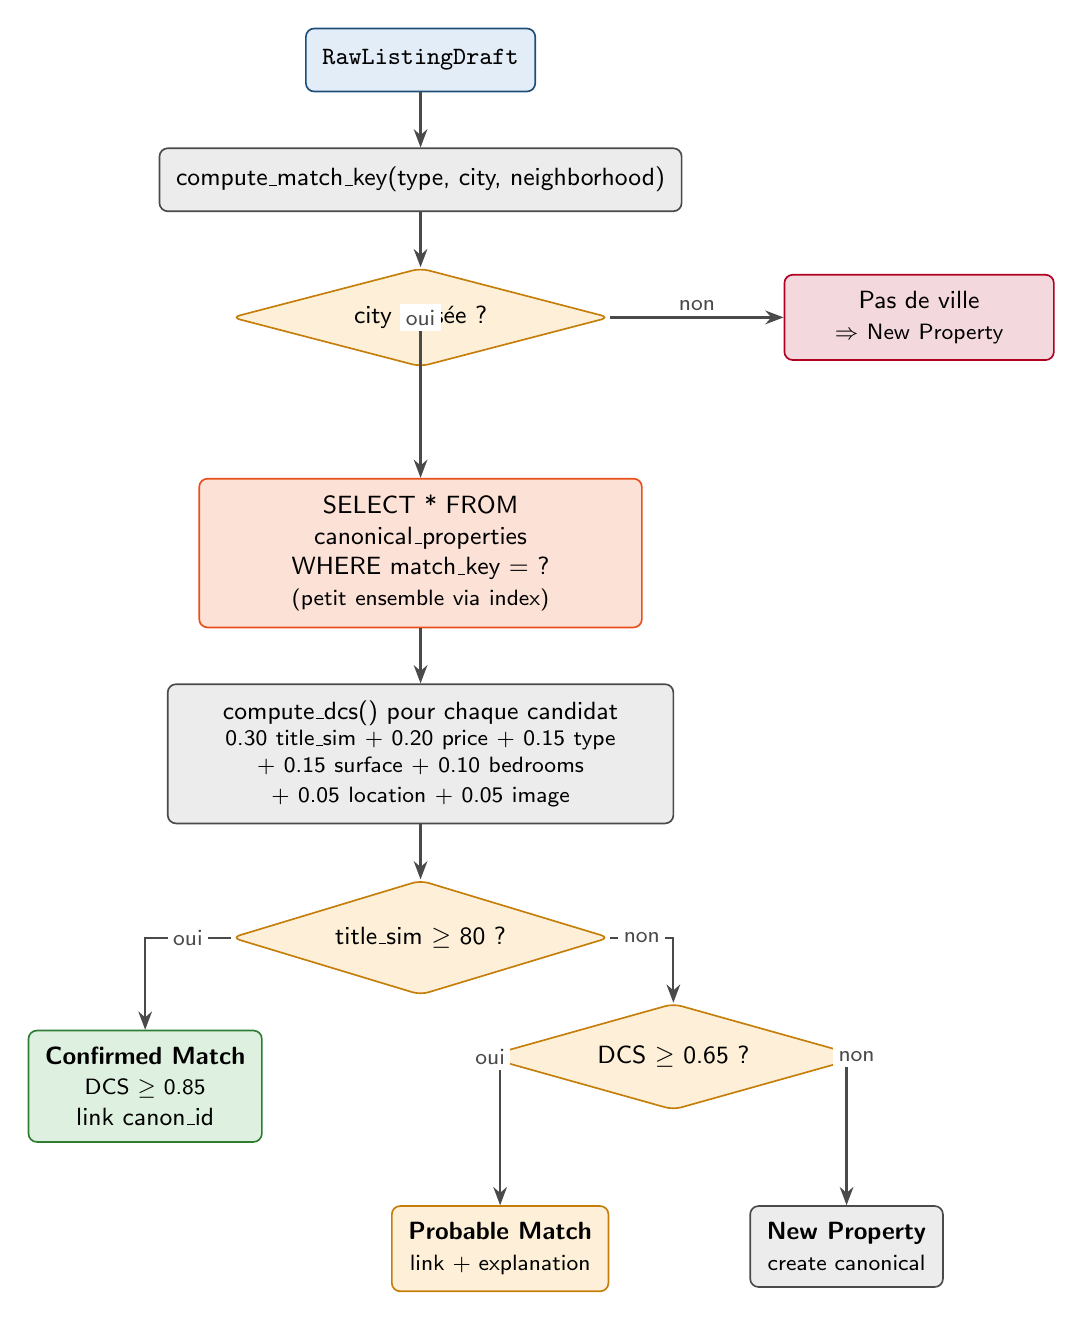
\begin{tikzpicture}[
  node distance=7mm,
  dec/.style={ci-amber, diamond, aspect=2.2, inner sep=2pt,
    minimum width=48mm, minimum height=12mm, font=\small\sffamily}
]
\node[ci-blue] (draft) {\texttt{RawListingDraft}};
\node[ci-gray, below=of draft] (key)
  {compute\_match\_key(type, city, neighborhood)};
\node[dec, below=of key] (haskey) {city pars\'ee ?};
\node[ci-orange, below=14mm of haskey, text width=52mm] (cand)
  {SELECT * FROM canonical\_properties\\ WHERE match\_key = ?\\
  \footnotesize (petit ensemble via index)};
\node[ci-gray, below=of cand, text width=60mm] (dcs)
  {compute\_dcs() pour chaque candidat\\
  \footnotesize 0.30 title\_sim + 0.20 price + 0.15 type\\
  \footnotesize + 0.15 surface + 0.10 bedrooms\\
  \footnotesize + 0.05 location + 0.05 image};
\node[dec, below=of dcs] (best) {title\_sim $\geq$ 80 ?};
\node[ci-green, below left=8mm and 8mm of best] (conf)
  {\textbf{Confirmed Match}\\ \footnotesize DCS $\geq$ 0.85\\ link canon\_id};
\node[dec, below right=8mm and 8mm of best] (prob) {DCS $\geq$ 0.65 ?};
\node[ci-amber, below=12mm of prob, xshift=-22mm] (p)
  {\textbf{Probable Match}\\ \footnotesize link + explanation};
\node[ci-gray, below=12mm of prob, xshift=22mm] (np)
  {\textbf{New Property}\\ \footnotesize create canonical};

\node[ci-box, draw=ciRed, fill=ciRed!15, right=22mm of haskey,
  text width=30mm] (noloc) {Pas de ville\\ \footnotesize $\Rightarrow$ New Property};

\draw[ci-flow] (draft) -- (key);
\draw[ci-flow] (key) -- (haskey);
\draw[ci-flow] (haskey) -| node[ci-label,pos=0.25]{oui} (cand);
\draw[ci-flow] (haskey) -- node[ci-label,above]{non} (noloc);
\draw[ci-flow] (cand) -- (dcs);
\draw[ci-flow] (dcs) -- (best);
\draw[ci-flow] (best) -| node[ci-label,pos=0.25]{oui} (conf);
\draw[ci-flow] (best) -| node[ci-label,pos=0.25]{non} (prob);
\draw[ci-flow] (prob) -| node[ci-label,pos=0.2]{oui} (p);
\draw[ci-flow] (prob) -| node[ci-label,pos=0.2]{non} (np);
\end{tikzpicture}
\caption{Arbre de d\'ecision du matcher DCS.}
\end{figure}

% ================================================================== %
\chapter{Scraper universel}
% ================================================================== %

Le scraper universel permet l'ajout d'un nouveau site en quelques minutes,
sans adaptateur d\'edi\'e. Quatre \'etapes~: d\'ecouverte d'URLs, d\'etection
de cartes, extraction multi-source, scoring de confiance.

\begin{figure}[H]
\centering
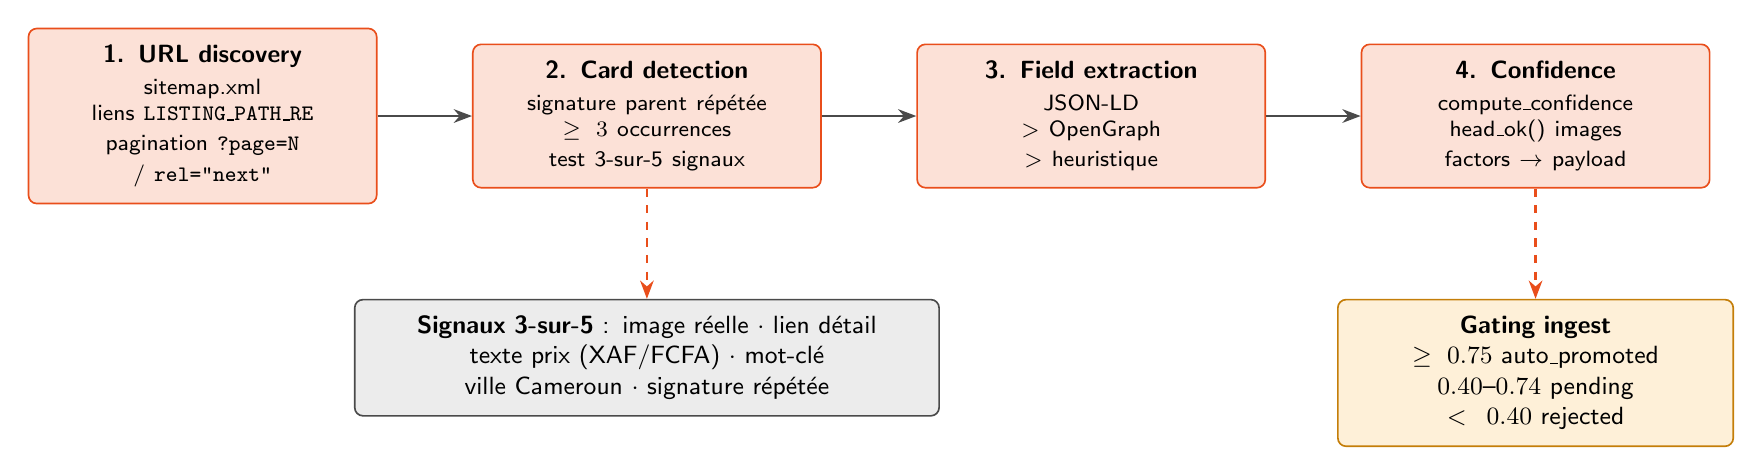
\begin{tikzpicture}[
  node distance=10mm,
  stage/.style={ci-orange, text width=40mm, minimum height=16mm,
    font=\small\bfseries\sffamily, align=center}
]
\node[stage] (s1) {1. URL discovery\\[2pt]
  \footnotesize\mdseries sitemap.xml\\
  liens \texttt{LISTING\_PATH\_RE}\\
  pagination \texttt{?page=N} / \texttt{rel="next"}};
\node[stage, right=12mm of s1] (s2) {2. Card detection\\[2pt]
  \footnotesize\mdseries signature parent r\'ep\'et\'ee\\
  $\geq 3$ occurrences\\
  test 3-sur-5 signaux};
\node[stage, right=12mm of s2] (s3) {3. Field extraction\\[2pt]
  \footnotesize\mdseries JSON-LD\\
  $>$ OpenGraph\\
  $>$ heuristique};
\node[stage, right=12mm of s3] (s4) {4. Confidence\\[2pt]
  \footnotesize\mdseries compute\_confidence\\
  head\_ok() images\\
  factors $\to$ payload};

\node[ci-gray, below=14mm of s2, text width=70mm] (signals)
  {\textbf{Signaux 3-sur-5}~: image r\'eelle $\cdot$ lien d\'etail\\
  texte prix (XAF/FCFA) $\cdot$ mot-cl\'e ville Cameroun $\cdot$ signature r\'ep\'et\'ee};

\node[ci-amber, below=14mm of s4, text width=46mm] (gate)
  {\textbf{Gating ingest}\\
  $\geq 0.75$ auto\_promoted\\
  $0.40$--$0.74$ pending\\
  $< 0.40$ rejected};

\draw[ci-flow] (s1) -- (s2);
\draw[ci-flow] (s2) -- (s3);
\draw[ci-flow] (s3) -- (s4);
\draw[ci-flow-d] (s2) -- (signals);
\draw[ci-flow-d] (s4) -- (gate);
\end{tikzpicture}
\caption{Pipeline en quatre \'etapes du scraper universel.}
\end{figure}

% ================================================================== %
\chapter{Pipeline analytique et scoring}
% ================================================================== %

\texttt{core/analytics.py:recompute\_all} parcourt toutes les
\texttt{locations}, calcule pour chacune (et par type de bien) des
agr\'egats de prix, des indicateurs de march\'e et cinq scores normalis\'es
0--10 produits par \texttt{core/scoring.py}. Le r\'esultat est upsert\'e dans
\texttt{neighborhood\_analytics}, lu ensuite par l'API
\texttt{GET /neighborhoods/\{slug\}}.

\begin{figure}[H]
\centering
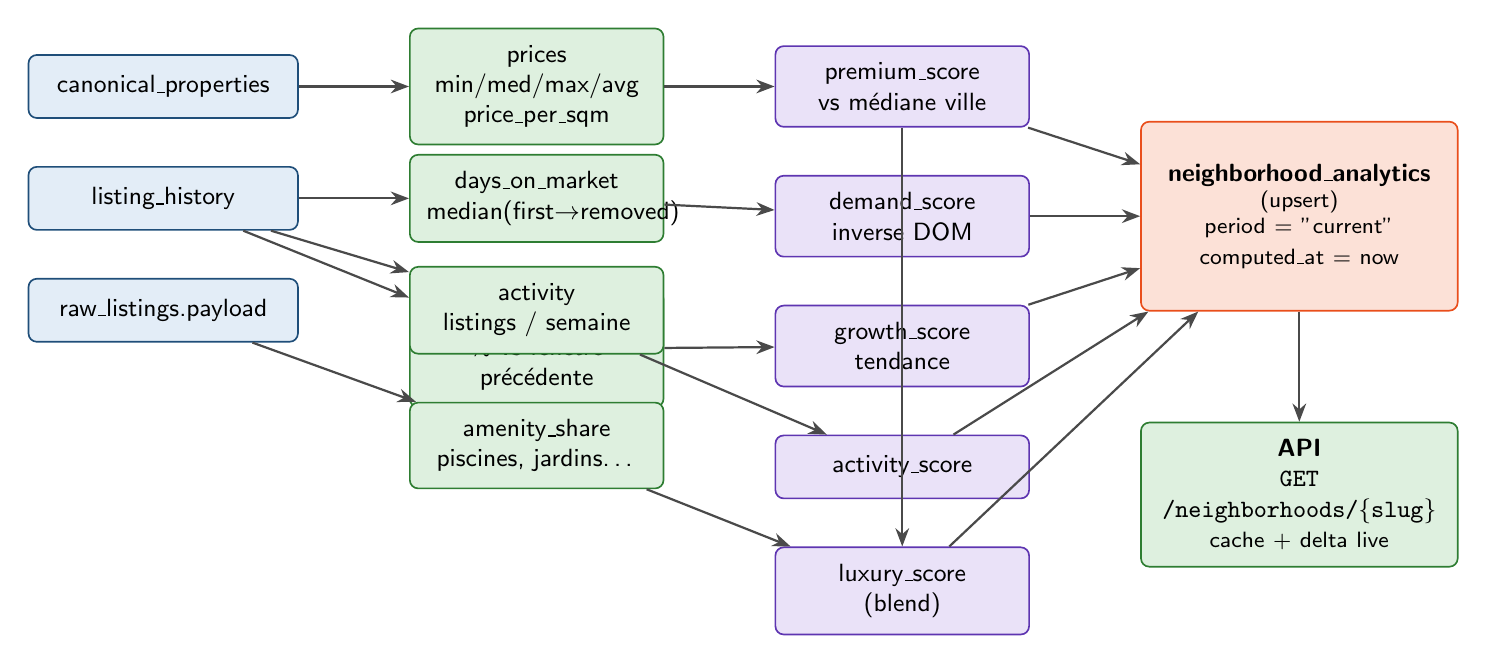
\begin{tikzpicture}[
  node distance=6mm and 12mm,
  src/.style={ci-blue, text width=30mm, minimum height=8mm},
  agg/.style={ci-green, text width=28mm, minimum height=8mm},
  sc/.style={ci-purple, text width=28mm, minimum height=8mm}
]
% Sources
\node[src] (canon) {canonical\_properties};
\node[src, below=of canon] (hist) {listing\_history};
\node[src, below=of hist] (raw) {raw\_listings.payload};

% Aggregats
\node[agg, right=14mm of canon] (prices)
  {prices\\ min/med/max/avg\\ price\_per\_sqm};
\node[agg, right=14mm of hist] (dom)
  {days\_on\_market\\ median(first$\to$removed)};
\node[agg, below=of dom] (trend)
  {trend 90j\\ \% vs fen\^etre pr\'ec\'edente};
\node[agg, right=14mm of raw] (act)
  {activity\\ listings / semaine};
\node[agg, below=of act] (amen)
  {amenity\_share\\ piscines, jardins\ldots};

% Scores
\node[sc, right=14mm of prices] (prem) {premium\_score\\ vs m\'ediane ville};
\node[sc, below=of prem] (dem) {demand\_score\\ inverse DOM};
\node[sc, below=of dem] (gro) {growth\_score\\ tendance};
\node[sc, below=of gro] (actS) {activity\_score};
\node[sc, below=of actS] (lux) {luxury\_score\\ (blend)};

% Cache
\node[ci-orange, right=14mm of dem, text width=36mm, minimum height=24mm]
  (cache) {\textbf{neighborhood\_analytics}\\ \footnotesize (upsert)\\
  \footnotesize period = "current"\\
  \footnotesize computed\_at = now};
\node[ci-green, below=14mm of cache, text width=36mm] (api)
  {\textbf{API}\\ \texttt{GET /neighborhoods/\{slug\}}\\ \footnotesize cache + delta live};

\draw[ci-flow] (canon) -- (prices);
\draw[ci-flow] (hist) -- (dom);
\draw[ci-flow] (hist) -- (trend);
\draw[ci-flow] (hist) -- (act);
\draw[ci-flow] (raw) -- (amen);
\draw[ci-flow] (prices) -- (prem);
\draw[ci-flow] (dom) -- (dem);
\draw[ci-flow] (trend) -- (gro);
\draw[ci-flow] (act) -- (actS);
\draw[ci-flow] (prem) -- (lux);
\draw[ci-flow] (amen) -- (lux);
\draw[ci-flow] (prem) -- (cache);
\draw[ci-flow] (dem) -- (cache);
\draw[ci-flow] (gro) -- (cache);
\draw[ci-flow] (actS) -- (cache);
\draw[ci-flow] (lux) -- (cache);
\draw[ci-flow] (cache) -- (api);
\end{tikzpicture}
\caption{Du brut au score~: pipeline de \texttt{recompute\_all}.}
\end{figure}

% ================================================================== %
\chapter{Flux de requ\^etes API}
% ================================================================== %

Les clients Flutter consomment l'API via Dio (\texttt{ApiClient}). Les
filtres sont appliqu\'es c\^ot\'e serveur (jamais en client). L'API FastAPI
monte cinq routeurs, chacun avec injection de \texttt{Session} SQLAlchemy.

\begin{figure}[H]
\centering
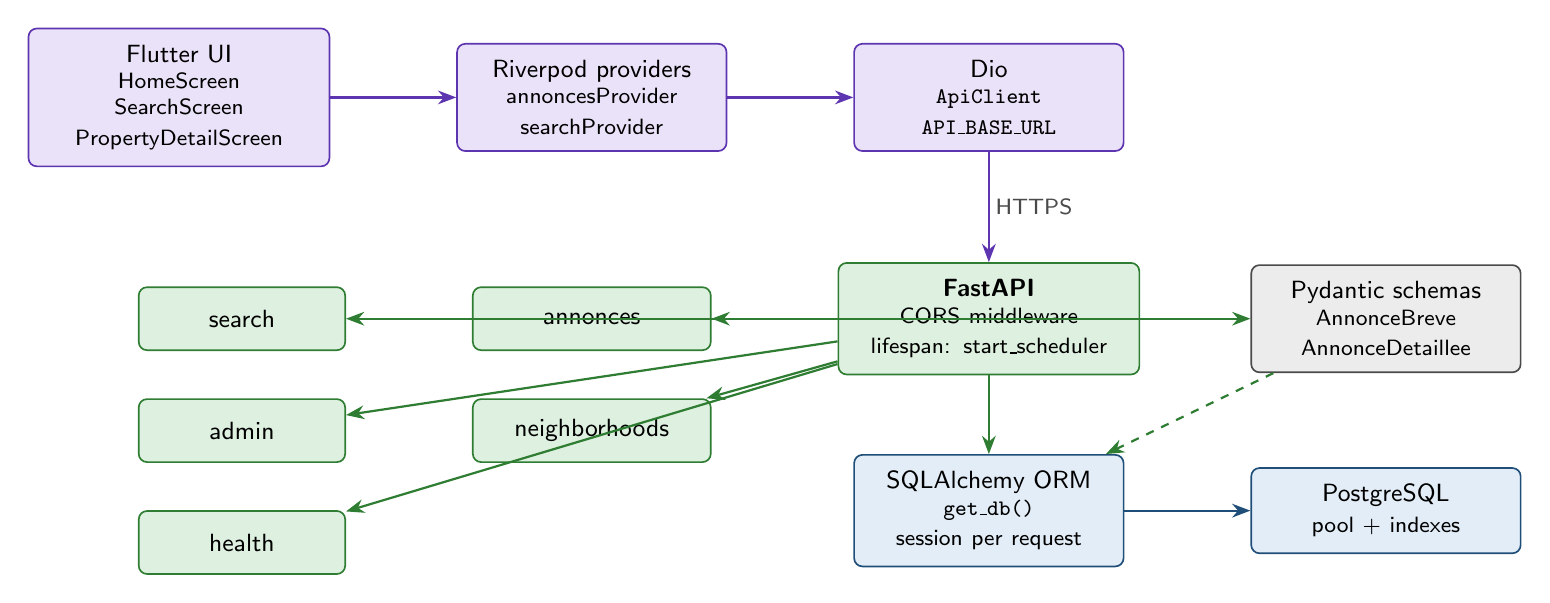
\begin{tikzpicture}[node distance=6mm and 16mm]
\node[ci-purple, text width=34mm] (ui) {Flutter UI\\ \footnotesize HomeScreen\\
  SearchScreen\\ PropertyDetailScreen};
\node[ci-purple, right=of ui, text width=30mm] (riverpod)
  {Riverpod providers\\ \footnotesize annoncesProvider\\ searchProvider};
\node[ci-purple, right=of riverpod, text width=30mm] (dio)
  {Dio \\ \footnotesize \texttt{ApiClient}\\ \texttt{API\_BASE\_URL}};

\node[ci-green, below=14mm of dio, text width=34mm] (fastapi)
  {\textbf{FastAPI}\\ \footnotesize CORS middleware\\ lifespan: start\_scheduler};
\node[ci-green, left=of fastapi, text width=26mm] (r1) {annonces};
\node[ci-green, left=of r1, text width=22mm] (r2) {search};
\node[ci-green, below=of r1, text width=26mm] (r3) {neighborhoods};
\node[ci-green, below=of r2, text width=22mm] (r4) {admin};
\node[ci-green, below=of r4, text width=22mm] (r5) {health};

\node[ci-gray, right=14mm of fastapi, text width=30mm] (schemas)
  {Pydantic schemas\\ \footnotesize AnnonceBreve\\ AnnonceDetaillee};
\node[ci-blue, below=10mm of fastapi, text width=30mm] (orm)
  {SQLAlchemy ORM\\ \footnotesize \texttt{get\_db()}\\ session per request};
\node[ci-blue, right=of orm, text width=30mm] (pg)
  {PostgreSQL\\ \footnotesize pool + indexes};

\draw[ci-flow, draw=ciPurple] (ui) -- (riverpod);
\draw[ci-flow, draw=ciPurple] (riverpod) -- (dio);
\draw[ci-flow, draw=ciPurple] (dio) -- node[ci-label,right]{HTTPS}
  (fastapi);
\draw[ci-flow, draw=ciGreen] (fastapi) -- (r1);
\draw[ci-flow, draw=ciGreen] (fastapi) -- (r2);
\draw[ci-flow, draw=ciGreen] (fastapi) -- (r3);
\draw[ci-flow, draw=ciGreen] (fastapi) -- (r4);
\draw[ci-flow, draw=ciGreen] (fastapi) -- (r5);
\draw[ci-flow, draw=ciGreen] (r1) -- (schemas);
\draw[ci-flow, draw=ciGreen] (fastapi) -- (orm);
\draw[ci-flow, draw=ciBlue] (orm) -- (pg);
\draw[ci-flow-d, draw=ciGreen] (schemas) -- (orm);
\end{tikzpicture}
\caption{Flux d'une requ\^ete de l'\'ecran Flutter jusqu'\`a PostgreSQL.}
\end{figure}

% ================================================================== %
\chapter{Machine \`a \'etats du review}
% ================================================================== %

Le \texttt{review\_status} d'un \texttt{raw\_listing} suit le cycle de vie
d'une annonce issue du scraper universel. Les sources d\'edi\'ees
(\texttt{dedicated}) entrent directement en \texttt{auto\_promoted}. Seul
l'admin peut d\'ecider de la promotion d'une annonce \texttt{pending} via
\texttt{POST /admin/review}.

\begin{figure}[H]
\centering
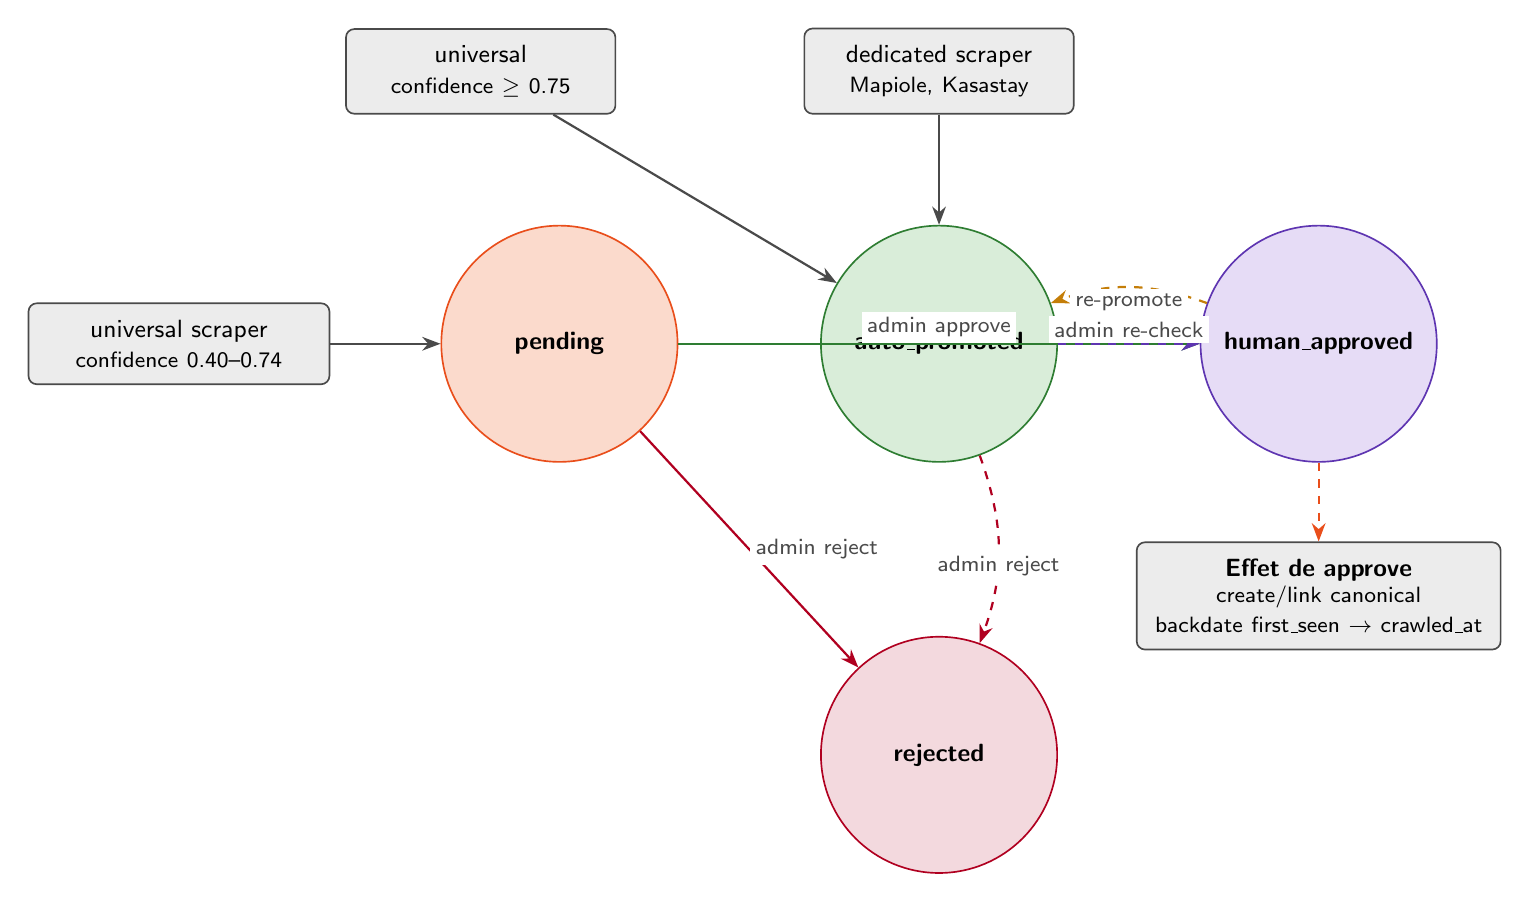
\begin{tikzpicture}[
  node distance=18mm,
  every state/.style={ci-box, draw=ciBlue, fill=ciBlueL!40,
    font=\small\bfseries\sffamily, minimum width=30mm, minimum height=12mm,
    align=center}
]
\node[state, fill=ciOrangeL!50, draw=ciOrange] (s0) {\textsc{pending}};
\node[state, fill=ciGreenL!70, draw=ciGreen, right=of s0] (s1)
  {\textsc{auto\_promoted}};
\node[state, fill=ciPurpleL!60, draw=ciPurple, right=of s1] (s2)
  {\textsc{human\_approved}};
\node[state, fill=ciRed!15, draw=ciRed, below=22mm of s1] (s3)
  {\textsc{rejected}};

\node[ci-gray, left=14mm of s0, text width=34mm] (src1)
  {universal scraper\\ \footnotesize confidence 0.40--0.74};
\node[ci-gray, above=14mm of s1, text width=30mm] (src2)
  {dedicated scraper\\ \footnotesize Mapiole, Kasastay};
\node[ci-gray, above=14mm of s0, xshift=-10mm, text width=30mm] (src3)
  {universal\\ \footnotesize confidence $\geq$ 0.75};

\draw[ci-flow] (src1) -- (s0);
\draw[ci-flow] (src2) -- (s1);
\draw[ci-flow] (src3) -- (s1);

\draw[ci-flow, draw=ciGreen] (s0) -- node[ci-label,above]
  {admin approve} (s2);
\draw[ci-flow, draw=ciRed] (s0) -- node[ci-label,right]
  {admin reject} (s3);
\draw[ci-flow-d, draw=ciPurple] (s1) -- node[ci-label,above]
  {admin re-check} (s2);
\draw[ci-flow-d, draw=ciRed] (s1) to[bend left=20] node[ci-label,below]
  {admin reject} (s3);
\draw[ci-flow-d, draw=ciAmber!80!black] (s2) to[bend right=20]
  node[ci-label,below]{re-promote} (s1);

\node[ci-gray, below=10mm of s2, text width=42mm] (eff)
  {\textbf{Effet de approve}\\ \footnotesize create/link canonical\\
  backdate first\_seen $\to$ crawled\_at};
\draw[ci-flow-d] (s2) -- (eff);
\end{tikzpicture}
\caption{Cycle de vie du \texttt{review\_status} d'un \texttt{raw\_listing}.}
\end{figure}

% ================================================================== %
\chapter{Synth\`ese et conventions cl\'es}
% ================================================================== %

\begin{itemize}[leftmargin=*, itemsep=2pt]
  \item \textbf{raw\_listings} est \emph{immutable}~: un re-crawl ne modifie
  jamais la ligne, il ajoute un \'ev\'enement dans \textbf{listing\_history}.
  \item \textbf{listing\_history} est \emph{append-only}~: aucun UPDATE,
  aucune suppression.
  \item \textbf{canonical\_properties.match\_key} est un bucket de
  r\'ecup\'eration de candidats, \emph{non unique}~; le DCS d\'esambigu\"ise.
  \item Les \textbf{pending} ne cr\'eent pas de canonical (\'evite les
  orphelins).
  \item Le \textbf{scheduler} vit dans le processus FastAPI
  (\texttt{APScheduler} BackgroundScheduler) et d\'eclenche~: crawl
  quotidien 02:00, refresh toutes les 6h, analytics hebdo lundi 03:00.
  \item Les scrapers respectent \textbf{robots.txt} via
  \texttt{BaseFetchMixin}, avec UA navigateur, jitter 2--5~s, retry
  exponentiel sur 429/5xx, d\'elai 15~s.
  \item Les filtres de l'API sont \emph{server-side}~; le client Flutter ne
  filtre jamais.
  \item L'\'etat Flutter est g\'er\'e par Riverpod, le routage par
  go\_router, l'HTTP par Dio avec \texttt{AppConfig.apiBaseUrl}.
  \item D\'eploiement AWS~: EC2 \texttt{t3.medium} pour l'app, RDS
  PostgreSQL multi-AZ, CloudFront pour le web et les images, Route~53 pour
  le DNS, Secrets Manager pour les credentials.
\end{itemize}

\end{document}